\subsection{Installation d'Hadoop:}
Apache Hadoop peut être installée dans différents modes selon l'exigence. Ces différents modes sont configurés lors de l'installation. Nous avons :

\begin{itemize}[label=\textbullet]
\item \textbf{Mode autonome:}C'est le mode de configuration par défaut d'Hadoop. Il n'utilise pas hdfs à la place, il utilise un système de fichiers local pour l'entrée et la sortie. Il est utile pour le  et les tests.
\item \textbf{ Mode pseudo-distribué}:Il est également appelé cluster à nœud unique où NameNode et DataNode résident sur la même machine. Tous les démons s'exécutent sur la même machine dans ce mode. Il produit un cluster entièrement fonctionnel sur une seule machine.
\item \textbf{Mode entièrement distribué:} Hadoop s'exécute sur plusieurs nœuds dans lesquels il existe des nœuds séparés pour les démons maîtres et esclaves. Les données sont réparties entre un cluster de machines fournissant un environnement de production.
\end{itemize}

Pour notre travail nous allons installer un cluster hadoop pseudo-distribué à nœud unique sur Windows 10.

\subsubsection{1. Prérequis:}
Tout d'abord, nous devons nous assurer que les prérequis suivants sont installés :

\begin{enumerate}
\item \textbf{Java 8 environnement d'exécution (JRE)}: Hadoop 3 nécessite une installation de Java 8. Je préfère utiliser le programme d' installation hors ligne. Lien de téléchargement \url{https://www.java.com/en/download/windows_offline.jsp}

\item \textbf{Java 8 development Kit (JDK)} Lien de téléchargement \url{https://www.oracle.com/java/technologies/downloads/#java8}

\item Pour décompresser les binaires Hadoop téléchargés, nous devons installer \textbf{7zip .} Lien de téléchargement \url{https://www.7-zip.org/download.html}
\end{enumerate}

\begin{figure}[h]
	\centering
    
\includegraphics[scale=0.6]{img/part3/1.3}
    \caption{Logo Java 8}
\end{figure}

\newpage
\subsubsection{2. Téléchargez les binaires Hadoop.}

\begin{enumerate}
\item La première étape consiste à télécharger les binaires Hadoop depuis le site officiel \url{https://archive.apache.org/dist/hadoop/common/hadoop-3.1.0/hadoop-3.1.0.tar.gz}.

\item Après avoir terminé le téléchargement du fichier, nous devons décompresser le package en utilisant 7zip en deux étapes. Tout d'abord, nous devons extraire la bibliothèque hadoop-3.1.0.tar.gz, puis nous devons décompresser le fichier tar extrait :
\begin{figure}[h]
	\centering
    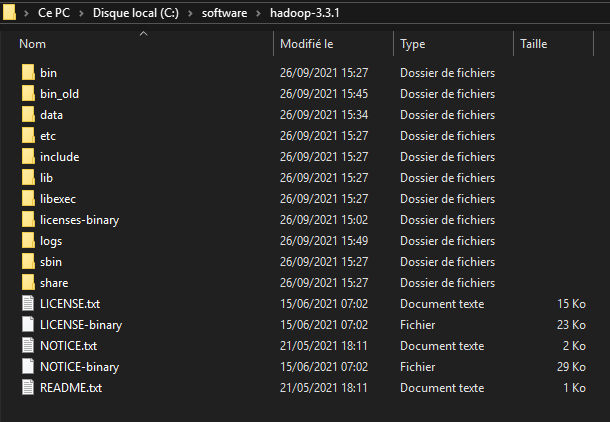
\includegraphics[scale=0.5]{img/part3/1.4}
    \caption{Les fichier Hadoop}
\end{figure}

\end{enumerate}

\subsubsection{3. Configuration Hadoop}
On doit impérativement maintenant éditer certains fichiers situés dans le répertoire hadoop du dossier 'etc' où nous avons installé hadoop. Les fichiers qui doivent être modifiés ont été mis en évidence:

\begin{enumerate}
\item On modifie le fichier \texttt{core-site.xml} dans le répertoire hadoop/etc/hadoop. On copie cette propriété xml dans la configuration dans le fichier:
\begin{figure}[h]
	\centering
    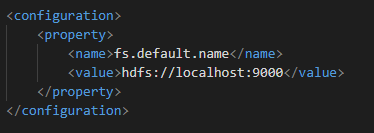
\includegraphics[scale=0.6]{img/part3/1.5}
    \caption{Modifier le fichier core-site.xml}
\end{figure}

\item On crée un dossier ‘data’ dans le répertoire hadoop. Puis on crée un dossier avec le nom ‘datanode’ et un dossier ‘namenode’ dans ce répertoire de données.
\begin{figure}[h]
	\centering
    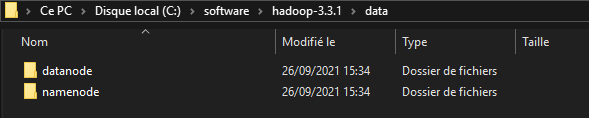
\includegraphics[scale=0.6]{img/part3/1.6}
    \caption{Créer les deux fichiers dans le dossier data}
\end{figure}

\newpage
\item On édite le fichier \texttt{hdfs-site.xml} dans le répertoire hadoop/etc/hadoop, et on ajoute la propriété ci-dessous dans la configuration:
\begin{figure}[h]
	\centering
    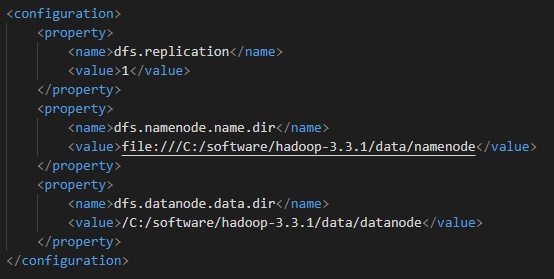
\includegraphics[scale=0.6]{img/part3/1.7}
    \caption{Modifier le fichier hdfs-site.xml}
\end{figure}

\item On modifie le fichier \texttt{yarn-site.xml} dans le répertoire hadoop/etc/hadoop, et on ajoute la propriété ci-dessous dans la configuration
\begin{figure}[h]
	\centering
    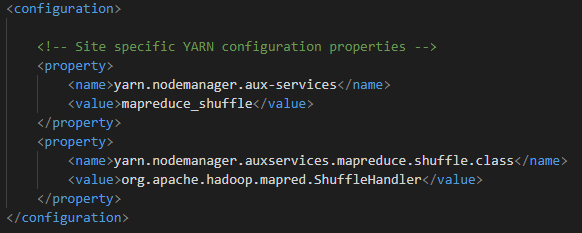
\includegraphics[scale=0.6]{img/part3/1.8}
    \caption{Modifier le fichier yarn-site.xml}
\end{figure}

\item On modifie \texttt{hadoop-env.cmd} et on remplace $JAVA HOME$ par le chemin du dossier java où la jdk 1.8 est installé.
\begin{figure}[h]
	\centering
    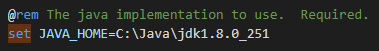
\includegraphics[scale=0.6]{img/part3/1.9}
    \caption{Modifier le fichier hadoop-env.cmd}
\end{figure}

\end{enumerate}

\newpage
\subsubsection{2. Configuration des variables d'environnement.}
\begin{enumerate}
\item On ouvre le panneau de configuration pour modifier la variable d'environnement système, pour créer une nouvelle variable utilisateur et Mettre le nom de variable comme $HADOOP HOME$ et la valeur de la variable comme chemin du dossier bin où on a extrait hadoop.
\begin{figure}[h]
	\centering
    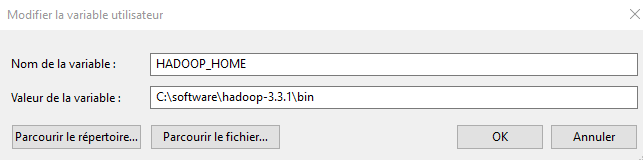
\includegraphics[scale=0.6]{img/part3/1.10}
    \caption{$HADOOP HOME$}
\end{figure}

\item De même, on crée une nouvelle variable utilisateur avec le nom de la variable comme $JAVA HOME$ et la valeur de la variable comme chemin du dossier bin dans le répertoire Java.
\begin{figure}[h]
	\centering
    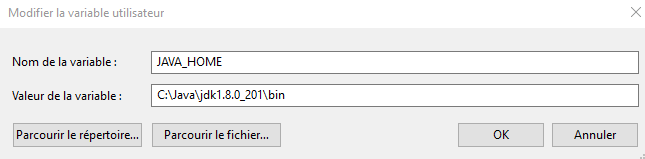
\includegraphics[scale=0.6]{img/part3/1.11}
    \caption{$JAVA HOME$}
\end{figure}

\item On doit maintenant définir le répertoire bin Hadoop et le chemin du répertoire bin Java dans le chemin de la variable système.

\end{enumerate}




























